\documentclass[11pt]{article}
\usepackage[margin=1in]{geometry}
\usepackage{amsmath,amssymb,amsthm}
\usepackage{physics}
\usepackage{booktabs}
\usepackage{graphicx}

\usepackage[colorlinks=true, linkcolor=blue, citecolor=blue, urlcolor=blue]{hyperref}
\usepackage{wasysym}
\usepackage{enumitem}
\usepackage{parskip}
\usepackage{xcolor}
\usepackage{float}
\usepackage{tikz}
\usepackage{tikz-3dplot}
\usetikzlibrary{calc,arrows.meta,positioning,decorations.pathreplacing,decorations.markings}

\newcommand{\vecr}{\vec r}
\newcommand{\vecL}{\vec L}
\newcommand{\vecA}{\vec A}
\newcommand{\vecf}{\vec f}
\newcommand{\vecF}{\vec F}
\newcommand{\vecp}{\vec p}
\newcommand{\vecx}{\vec x}
\newcommand{\hatn}{\hat \leo}
\newcommand{\rhat}{\hat r}
\newcommand{\phihat}{\hat\phi}
\newcommand{\note}[1]{\textcolor{blue!60!black}{\textit{[#1]}}}

\title{The Kepler Problem and Orbital Perturbation Theory}
\author{}
\date{}

\begin{document}
\maketitle

\tableofcontents

\section{The Two-Body Problem}

\subsection{Central force problem}
A central force acts along the line joining two particles and depends only on their separation $r=|\vecx_1-\vecx_2|$. Such a force is a gradient of a scalar potential $V(r)$:
\[
\vecF(\vecx_1,\vecx_2) = \nabla V(r).
\]
Newton's equations for the pair are
\begin{equation}
\frac{d^2}{dt^2}\begin{bmatrix}m_1 & 0\\0&m_2\end{bmatrix}\begin{bmatrix}\vecx_1\\\vecx_2\end{bmatrix}
=\begin{bmatrix}-\nabla V(r)\\ \nabla V(r)\end{bmatrix}. \label{eq:eom2}
\end{equation}
Six second-order ODEs $\Rightarrow$ 12 constants of integration in the general solution.

\subsection{Separating centre-of-mass motion}
With $M=m_1+m_2$, $\mu = m_1m_2/M$, transform to relative and centre-of-mass coordinates,
\[
\begin{bmatrix}\vecr\\ \vec X\end{bmatrix}=\begin{bmatrix}1&-1\\ m_1/M& m_2/M\end{bmatrix}\begin{bmatrix}\vecx_1\\\vecx_2\end{bmatrix},
\qquad
\begin{bmatrix}\vecx_1\\\vecx_2\end{bmatrix}=\begin{bmatrix}m_2/M&1\\-m_1/M&1\end{bmatrix}\begin{bmatrix}\vecr\\\vec X\end{bmatrix}.
\]
Substituting into \eqref{eq:eom2} and left-multiplying by $\begin{bmatrix}m_2/M&-m_1/M\\1&1\end{bmatrix}$ diagonalizes the mass matrix and decouples the two sectors:
\begin{align}
\mu\,\ddot{\vecr} &= -\nabla V(r), \label{eq:relEOM}\\
M\,\ddot{\vec X} &= 0. \label{eq:comEOM}
\end{align}
Equation \eqref{eq:comEOM} integrates trivially: $\vec X(t) = (\vec P/M)t+\vec X_0$, with $\vec P,\vec X_0$ six constants fixing the inertial frame in which the barycentre is at rest at the origin. Everything of dynamical interest is in the \emph{relative} coordinate $\vecr$, governed by \eqref{eq:relEOM} — a one-body central-force problem with reduced mass $\mu$.

\subsection{Conserved quantities}

\paragraph{Angular momentum.} Define $\vecL=\vecr\times\vecp=\mu\,\vecr\times\dot{\vecr}$. Then, because we are considering central force $\ddot{\vec r}\propto \hat{r}$ and hence,
\[
\dot{\vecL} = \mu\big[\dot{\vecr}\times\dot{\vecr}+\vecr\times\ddot{\vecr}\big]=0.
\]
$\vecL$ supplies three constants of motion: its magnitude $L$, and two angles fixing its direction — the \textbf{inclination} $\iota$ and \textbf{longitude of ascending node} $\Omega$ (Euler angles of the orbital plane relative to a reference plane). Conservation of $\vecL$ confines the motion to the plane $\perp\vecL$.
	
\paragraph{Energy.} $E=K+V$ with $K=\tfrac12\mu\dot{\vecr}^2$ (the centre-of-mass kinetic term is a constant and drops out). Then
\[
\dot E = \mu\dot{\vecr}\cdot\ddot{\vecr}+\dot V
=\mu\dot{\vecr}\cdot\ddot{\vecr}+\nabla V\cdot\dot{\vecr}
=\big(\mu\ddot{\vecr}+\nabla V\big)\cdot\dot{\vecr}=0
\]
by \eqref{eq:relEOM}. So $E$ is conserved for \emph{any} central potential $V(r)$, not just gravity.

\section{Coordinate Systems and Orbital Elements}

Fix an equatorial (reference) frame with $\hat\Upsilon$ (vernal equinox / first point of Aries) along $X$ and celestial north $\hat N$ along $Z$; $\hat Y$ completes the right-handed triad. For a source at $(\mathrm{RA},\mathrm{DEC})=(\alpha,\delta)$ the line of sight is
\[
\hat R = \cos\delta\cos\alpha\,\hat\Upsilon+\cos\delta\sin\alpha\,\hat Y+\sin\delta\,\hat N,
\]
with in-sky-plane axes (pointing along increasing RA, DEC)
\[
\hat\alpha=\frac{\pdv{\hat R}{\alpha}}{\abs{\pdv{\hat R}{\alpha}}}=-\sin\alpha\,\hat\Upsilon+\cos\alpha\,\hat Y,\qquad
\hat\delta=\frac{\pdv{\hat R}{\delta}}{\abs{\pdv{\hat R}{\delta}}}=-\sin\delta\cos\alpha\,\hat\Upsilon-\sin\delta\sin\alpha\,\hat Y+\cos\delta\,\hat N.
\]

The orbital plane has its own frame: origin at the barycentre, $X$-axis along the \textbf{line of nodes} (through the ascending node and the descending node), $Z$-axis along $\vecL$. Denote the unit vector towards the ascending node by $\hatn$. Then

\begin{align}
    \begin{pmatrix} \hatn\\ \hat y\\ \hat L \end{pmatrix} = 
    \begin{pmatrix} 1&0&0\\ 0&\cos\iota&\sin\iota\\ 0&-\sin\iota&\cos\iota \end{pmatrix} \begin{pmatrix} \cos\Omega&\sin\Omega&0\\ -\sin\Omega&\cos\Omega&0\\ 0&0&1 \end{pmatrix} \begin{pmatrix} \hat\alpha\\ \hat\delta\\ \hat R \end{pmatrix}.
\end{align}
Hence,
\begin{align}
\hatn  &= \cos\Omega\,\hat\alpha+\sin\Omega\,\hat\delta, \label{eq:node}\\
\hat y &= -\sin\Omega\cos\iota\,\hat\alpha+\cos\Omega\cos\iota\,\hat\delta+\sin\iota\,\hat R, \label{eq:yhat}\\
\hat L &= \sin\Omega\sin\iota\,\hat\alpha-\cos\Omega\sin\iota\,\hat\delta+\cos\iota\,\hat R, \label{eq:Lhat}
\end{align}
\begin{figure}[H]
    \centering
    	\tdplotsetmaincoords{70}{120}
         \resizebox{\textwidth}{!}{
	\begin{tikzpicture}[tdplot_main_coords, scale=3]
		
		%------------------------------------------------
		% Parameters
		%------------------------------------------------
		\def\a{2.7}
		\def\e{0.45}
		\def\inc{35}
		\def\Om{35}
		\def\om{20}
		
		% Position of the whole orbit
		\def\Ox{0.0}
		\def\Oy{0.0}
		\def\Oz{0.0}
		
		% Point to mark
		\def\numark{55}
		
		%------------------------------------------------
		% Sky plane
		%------------------------------------------------
		\fill[blue!5]
		(-4.5,-3.8,0) --
		( 4.5,-3.8,0) --
		( 4.5, 3.8,0) --
		(-4.5, 3.8,0) -- cycle;
		
		% X,Y axes: reference / sky plane
		\draw[->,blue!70!black]
		(-4.5,0,0) -- (4.8,0,0)
		node[anchor=north east] {$\hat\delta$};
		
		\draw[->,blue!70!black]
		(0,4.2,0) -- (0,-3.8,0)
		node[anchor=south] {$\hat\alpha$};
		
		% Z axis
		\draw[->,gray!70!black]
		(0,0,-1.5) -- (0,0,3.0)
		node[anchor=south west] {$Z$};
		
		\node[blue!60!black] at (3.2,3.2,0)
		{\small sky plane};
		
		%------------------------------------------------
		% Origin / centre of orbit
		%------------------------------------------------
		
		\fill (\Ox,\Oy,\Oz) circle (1.5pt);
		
		\node[above left] at (\Ox,\Oy,\Oz) {$O$};
		
		%------------------------------------------------
		% Omega
		% Angle from +alpha-hat toward +delta-hat
		%------------------------------------------------
		
		\draw[thick,blue!70!black,->]
		plot[
		variable=\theta,
		domain=-90:\Om,
		samples=40
		]
		(
		{\Ox+0.65*cos(\theta)},
		{\Oy+0.65*sin(\theta)},
		{\Oz}
		);
		
	
		\node[blue!70!black] at
		({\Ox+0.85*cos(\Om/2)},
		{\Oy+0.85*sin(\Om/2)},0)
		{$\Omega$};
		%------------------------------------------------
		% Actual inclined ellipse
		% Orbital plane
		%------------------------------------------------
		
		\draw[thick,red!70!black]
		plot[
		variable=\nu,
		domain=0:360,
		samples=250,
		smooth
		]
		(
		{
			\Ox+
			(\a*(1-\e*\e)/(1+\e*cos(\nu)))
			*
			(
			cos(\Om)*cos(\om+\nu)
			-sin(\Om)*cos(\inc)*sin(\om+\nu)
			)
		},
		{
			\Oy+
			(\a*(1-\e*\e)/(1+\e*cos(\nu)))
			*
			(
			sin(\Om)*cos(\om+\nu)
			+cos(\Om)*cos(\inc)*sin(\om+\nu)
			)
		},
		{
			\Oz+
			(\a*(1-\e*\e)/(1+\e*cos(\nu)))
			*
			(
			sin(\inc)*sin(\om+\nu)
			)
		}
		);
		
		%------------------------------------------------
		% Projected ellipse
		% Lies in XY sky plane
		%------------------------------------------------
		
		\draw[very thick,dashed,blue!45!black]
		plot[
		variable=\nu,
		domain=0:360,
		samples=250,
		smooth
		]
		(
		{
			\Ox+
			(\a*(1-\e*\e)/(1+\e*cos(\nu)))
			*
			(
			cos(\Om)*cos(\om+\nu)
			-sin(\Om)*cos(\inc)*sin(\om+\nu)
			)
		},
		{
			\Oy+
			(\a*(1-\e*\e)/(1+\e*cos(\nu)))
			*
			(
			sin(\Om)*cos(\om+\nu)
			+cos(\Om)*cos(\inc)*sin(\om+\nu)
			)
		},
		0
		);
		
		%------------------------------------------------
		% Periapsis
		%------------------------------------------------
		
		\pgfmathsetmacro{\rp}{\a*(1-\e)}
		
		\pgfmathsetmacro{\periX}
		{\Ox+\rp*(cos(\Om)*cos(\om)
			-sin(\Om)*cos(\inc)*sin(\om))}
		
		\pgfmathsetmacro{\periY}
		{\Oy+\rp*(sin(\Om)*cos(\om)
			+cos(\Om)*cos(\inc)*sin(\om))}
		
		\pgfmathsetmacro{\periZ}
		{\Oz+\rp*sin(\inc)*sin(\om)}
		
		% Direction to periapsis
		\draw[thick,red!70!black,->]
		(\Ox,\Oy,\Oz)
		-- (\periX,\periY,\periZ);
		
		% Periapsis point
		\fill[red!70!black]
		(\periX,\periY,\periZ) circle (2pt);
		
		\node[red!70!black,above right] at
		(\periX,\periY,\periZ)
		{periapsis};
		
		%------------------------------------------------
		% omega
		% Angle in orbital plane
		%------------------------------------------------
		
		\def\Romega{0.75}
		
		\draw[thick,red!70!black,->]
		plot[
		variable=\theta,
		domain=0:\om,
		samples=30
		]
		(
		{
			\Ox+\Romega*
			(
			cos(\Om)*cos(\theta)
			-sin(\Om)*cos(\inc)*sin(\theta)
			)
		},
		{
			\Oy+\Romega*
			(
			sin(\Om)*cos(\theta)
			+cos(\Om)*cos(\inc)*sin(\theta)
			)
		},
		{
			\Oz+\Romega*sin(\inc)*sin(\theta)
		}
		);
		
		\node[red!70!black] at
		(
		{
			\Ox+1.0*
			(
			cos(\Om)*cos(\om/2)
			-sin(\Om)*cos(\inc)*sin(\om/2)
			)
		},
		{
			\Oy+1.0*
			(
			sin(\Om)*cos(\om/2)
			+cos(\Om)*cos(\inc)*sin(\om/2)
			)
		},
		{
			\Oz+1.0*sin(\inc)*sin(\om/2)
		}
		)
		{$\omega$};
		
		%------------------------------------------------
		% Inclination I
		% Angle between reference and orbital planes
		%------------------------------------------------
		
		\def\Rinc{1.5}
		
		% Reference-plane direction
		\coordinate (A) at
		({\Rinc*cos(\Om)},
		{\Rinc*sin(\Om)},0);
		
		% Corresponding direction in orbital plane
		\coordinate (B) at
		({\Rinc*cos(\Om)-1.0*sin(\Om)*cos(\inc)},
		{\Rinc*sin(\Om)+1.0*cos(\Om)*cos(\inc)},
		{1.0*sin(\inc)});
		
		% Direction in reference plane
		\coordinate (C) at
		({\Rinc*cos(\Om)-1.0*sin(\Om)},
		{\Rinc*sin(\Om)+1.0*cos(\Om)},0);
		
		% Show the two planes locally
		\draw[blue!50!black,dashed] (A) -- (C);
		\draw[red!50!black,dashed] (A) -- (B);
		
		% Arc representing inclination
		\draw[thick,red!70!black,->]
		plot[
		variable=\theta,
		domain=0:\inc,
		samples=30
		]
		(
		{\Rinc*cos(\Om)-0.55*sin(\Om)*cos(\theta)},
		{\Rinc*sin(\Om)+0.55*cos(\Om)*cos(\theta)},
		{0.55*sin(\theta)}
		);
		
		\node[red!70!black] at
		(
		{\Rinc*cos(\Om)-0.72*sin(\Om)*cos(\inc/2)},
		{\Rinc*sin(\Om)+0.72*cos(\Om)*cos(\inc/2)},
		{0.72*sin(\inc/2)}
		)
		{$I$};
		
		%------------------------------------------------
		% Mark a point P on the actual orbit
		%------------------------------------------------
		
		\pgfmathsetmacro{\rr}
		{\a*(1-\e*\e)/(1+\e*cos(\numark))}
		
		\pgfmathsetmacro{\PX}
		{\Ox+\rr*(cos(\Om)*cos(\om+\numark)
			-sin(\Om)*cos(\inc)*sin(\om+\numark))}
		
		\pgfmathsetmacro{\PY}
		{\Oy+\rr*(sin(\Om)*cos(\om+\numark)
			+cos(\Om)*cos(\inc)*sin(\om+\numark))}
		
		\pgfmathsetmacro{\PZ}
		{\Oz+\rr*sin(\inc)*sin(\om+\numark)}
		
		% Point on orbit
		\fill[red!70!black]
		(\PX,\PY,\PZ) circle (2pt);
		
		\node[red!70!black,above right] at
		(\PX,\PY,\PZ) {$P$};
		
		%------------------------------------------------
		% Projection of P onto sky plane
		%------------------------------------------------
		
		\fill[blue!70!black]
		(\PX,\PY,0) circle (2pt);
		
		\node[blue!70!black,below right] at
		(\PX,\PY,0) {$P_{\rm sky}$};
		
		% Projection line
		\draw[gray,dotted,thick]
		(\PX,\PY,\PZ) -- (\PX,\PY,0);
		
		%------------------------------------------------
		% Direction from O to P
		%------------------------------------------------
		
		\draw[red!40!black,dashed]
		(\Ox,\Oy,\Oz) -- (\PX,\PY,\PZ);
		
		%------------------------------------------------
		% nu
		% Angle from periapsis to P
		% in orbital plane
		%------------------------------------------------
		
		\def\Rnu{1.05}
		
		\draw[thick,red!70!black,->]
		plot[
		variable=\theta,
		domain=\om:\om+\numark,
		samples=50,
		smooth
		]
		(
		{
			\Ox+\Rnu*
			(
			cos(\Om)*cos(\theta)
			-sin(\Om)*cos(\inc)*sin(\theta)
			)
		},
		{
			\Oy+\Rnu*
			(
			sin(\Om)*cos(\theta)
			+cos(\Om)*cos(\inc)*sin(\theta)
			)
		},
		{
			\Oz+\Rnu*sin(\inc)*sin(\theta)
		}
		);
		
		\node[red!70!black] at
		(
		{
			\Ox+1.25*
			(
			cos(\Om)*cos(\om+\numark/2)
			-sin(\Om)*cos(\inc)*sin(\om+\numark/2)
			)
		},
		{
			\Oy+1.25*
			(
			sin(\Om)*cos(\om+\numark/2)
			+cos(\Om)*cos(\inc)*sin(\om+\numark/2)
			)
		},
		{
			\Oz+1.25*sin(\inc)*sin(\om+\numark/2)
		}
		)
		{$\nu$};
        	%------------------------------------------------
		% Orbital-plane basis vectors
		%------------------------------------------------
		
		\def\Ry{2.0}
		\def\RL{2.4}
		
		%------------------------------------------------
		% y-hat
		%
		% y-hat =
		% -sin(Omega) cos(i) X
		% +cos(Omega) cos(i) Y
		% +sin(i) Z
		%------------------------------------------------
		
		\pgfmathsetmacro{\yX}
		{\Ox-\Ry*sin(\Om)*cos(\inc)}
		
		\pgfmathsetmacro{\yY}
		{\Oy+\Ry*cos(\Om)*cos(\inc)}
		
		\pgfmathsetmacro{\yZ}
		{\Oz+\Ry*sin(\inc)}
		
		\coordinate (Yhat) at (\yX,\yY,\yZ);
		
		\draw[
		very thick,
		purple!80!black,
		->,
		>=stealth
		]
		(\Ox,\Oy,\Oz) -- (Yhat)
		node[above right] {$\hat y$};
		
		
		%------------------------------------------------
		% L-hat
		%
		% L-hat = n-hat x y-hat
		%
		% L-hat =
		% +sin(Omega) sin(i) X
		% -cos(Omega) sin(i) Y
		% +cos(i) Z
		%------------------------------------------------
		
		\pgfmathsetmacro{\LX}
		{\Ox+\RL*sin(\Om)*sin(\inc)}
		
		\pgfmathsetmacro{\LY}
		{\Oy-\RL*cos(\Om)*sin(\inc)}
		
		\pgfmathsetmacro{\LZ}
		{\Oz+\RL*cos(\inc)}
		
		\coordinate (Lhat) at (\LX,\LY,\LZ);
		
		\draw[
		very thick,
		red!70!black,
		->,
		>=stealth
		]
		(\Ox,\Oy,\Oz) -- (Lhat)
		node[above right] {$\hat L$};
        %------------------------------------------------
		% Line of ascending node
		% Reference-plane quantity
		%------------------------------------------------
		
		\draw[very thick,red!70!black,->](\Ox,\Oy,\Oz)-- ({\Ox+2.4*cos(\Om)},{\Oy+2.4*sin(\Om)},\Oz)node[right] {$\hatn$};
		
	\end{tikzpicture}}
    \caption{Orientation of an orbit relative to sky plane. $\Omega$ (longitude of ascending node) is measured from the reference direction $\alpha$ to the ascending node along the sku plane; $\omega$ (argument of periapsis) is measured from the ascending node to perigee \emph{within} the orbital plane; $\iota$ (inclination) is the dihedral angle between the two planes, read off at the node; $\nu$ (true anomaly) is measured from perigee to the heavenly body's current position. This is exactly $(\Omega,\iota,\omega)$ of Eqs.~\eqref{eq:node}--\eqref{eq:yhat} describe.}
\label{fig:elements}
\end{figure}
so that $\iota=\arccos(\hat L\cdot\hat R)$ is the angle between orbital and reference planes, and $(\hatn,\hat y,\hat L)$ is a right-handed orthonormal triad spanning the orbital plane plus its normal. In this plane use polar coordinates $(r,\phi)$ measured from $\hatn$:

\begin{equation}
\rhat=\cos\phi\,\hatn+\sin\phi\,\hat y,\qquad
\phihat=-\sin\phi\,\hatn+\cos\phi\,\hat y. \label{eq:rhat_phihat}
\end{equation}
\paragraph{The projected orbit in the sky plane}: If the object in its orbital plane as the coordinate $(r\cos(\omega+\nu),r\sin(\omega+\nu))$, the corresponding coordinate in the sky plane could be found as:

	\begin{align}
		\begin{pmatrix}
			X \\
			Y \\
			Z
		\end{pmatrix}_{\text{Sky Plane}}= 
		\begin{pmatrix}
			\cos\Omega & -\sin\Omega & 0 \\
			\sin\Omega & \cos\Omega & 0 \\
			0 & 0 & 1
		\end{pmatrix}
		\begin{pmatrix}
			1 & 0 & 0 \\
			0 & \cos i & -\sin i \\
			0 & \sin i & \cos i
		\end{pmatrix}
		\begin{pmatrix}
			r\cos(\omega+\nu) \\
			r\sin(\omega+\nu) \\
			0
		\end{pmatrix}_{\text{Orbital Plane}}.
	\end{align}
    Then,
    \begin{align}
X &= r\left(\cos(\omega+\nu)\cos\Omega-\sin (\omega+\nu)\sin\Omega\cos i\right),\\
Y &= r\left(\cos(\omega+\nu)\sin\Omega+\sin (\omega+\nu)\cos\Omega\cos i\right).
\end{align}
	\begin{figure}[H]
	\centering
	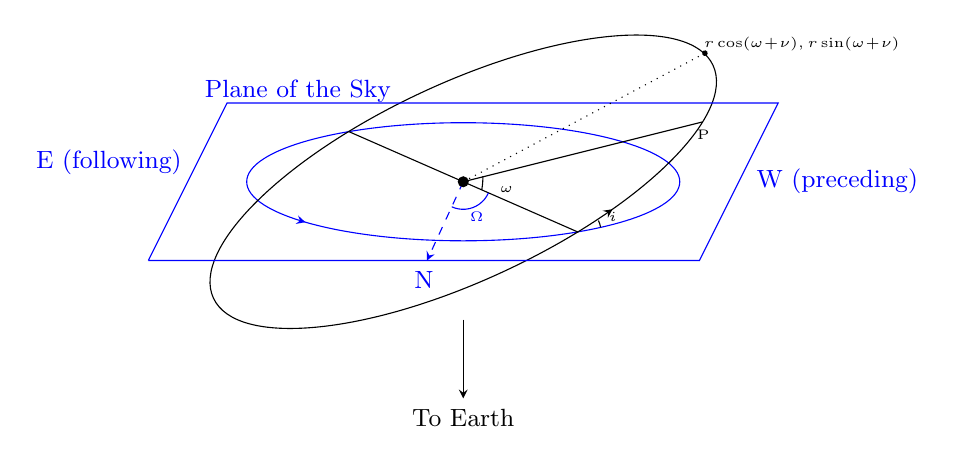
\begin{tikzpicture}
		\draw[blue,postaction={decorate,	decoration={markings,mark=at position 0.58 with {\arrow[>=stealth]{>}}}}] (0,0) ellipse (2.75 and 0.75);
		\draw[rotate=25,postaction={decorate,	decoration={markings,mark=at position 0.85 with {\arrow[>=stealth]{>}}}}] (0,0) ellipse (3.5 and 1.25);
		\draw [blue] (-4,-1)--(-3,1)--(4,1)--(3,-1)--(-4,-1);
		\draw (1.46,-0.64)--(-1.46,0.64);
		\draw (0,0)--(3.04,0.76);
		\draw [dashed,->,>=stealth,blue](0,0)--(-0.46,-1);
		\fill[black] (0,0) circle (2pt);
		\draw[->,>=stealth] (0,-1.75)--(0,-2.75);
		\draw [-{Circle[length=2pt]}, dotted] (0,0) -- (3.1, 1.65);
		\small
		\node at (0,-3) {To Earth};
		\node[blue] at (-0.5,-1.25) {N};
		\node[blue] at (-4.5,0.25) {E (following)};
		\node[blue] at (-2.1,1.15) {Plane of the Sky};
		\node[blue] at (4.75,0) {W (preceding)};
		\tiny
		\node at (4.3,1.75) {$r\cos(\omega\!+\!\nu), r\sin(\omega\!+\!\nu)$};
		\node at (3.05,0.6) {P};
		\draw (1.4,-0.64) ++(10:0.35) arc[start angle=10,end angle=25,radius=0.35];
		\node at (1.9,-0.45) {$i$};
		\node[black] at (0.55,-0.1) {$\omega$};
		\draw (0.25,0.07) arc [start angle=0, end angle=-10, radius=1];
		\draw[blue] (-114.7:0.35) arc[start angle=-114.7, end angle=-23.7, radius=0.35];
		\node[blue] at (-69.2:0.48) {$\Omega$};
	\end{tikzpicture}
	\caption{In this North becomes the local $X$ axis and West becomes the $Y$ axis of the sky plane.}	
\end{figure}

One can set $\Omega=0$ by another set of basis in the sky plane and then the analysis simplifies immensely
\begin{align}
X &= r\cos(\omega+\nu),\\
Y &= r\sin (\omega+\nu)\cos i.
\end{align}
We find that the semi minor axis shrinks by the factor of $\cos i$.
\paragraph{The six orbital elements.} As the orbit solution unfolds below, six constants emerge in total: $\Omega,\iota$ (orientation of the plane, from $\vecL$), $a,e$ (size and shape, from $E,L$), $\omega$ (orientation of the ellipse \emph{within} the plane, the \textbf{argument of periapsis}), and $T_0$ (time of periapsis passage, fixing where on the ellipse the body is at a given time). Figure~\ref{fig:elements} shows all of these together.

\section{Planar Motion and Kepler's Second Law}

\paragraph{Areal velocity.} The area swept by $\vecr$ in time $dt$ is $dA=\int_{0}^{2\pi}\int_{0}^{r(\phi)} r drd\phi=\frac{1}{2}\int_{0}^{2\pi}r^2(\phi)d\phi$, so
\begin{equation}
\frac{dA}{dt}=\frac{r^2\dot\phi}{2} = \frac{L}{2\mu} = \text{const.} \label{eq:kepler2}
\end{equation}
This is \textbf{Kepler's second law}: equal areas in equal times. It follows purely from $\vecL$ being conserved, i.e.\ from the force being central — no dependence on the specific form of $V(r)$.

\paragraph{Equations of motion in $(r,\phi)$.} With $Z\parallel\vecL$ and $X\parallel\hatn$, $\vecr=r\rhat$, and
\[
\dot{\vecr}=\dot r\,\rhat+r\dot{\hat{r}}=\dot r\,\rhat+r\dot\phi\,\phihat,\qquad
\ddot{\vecr}=\big(\ddot r-r\dot\phi^2\big)\rhat+\big(2\dot r\dot\phi+r\ddot\phi\big)\phihat.
\]
where we used $\nabla_{\mu}\mathbf{e}_{\nu}=\Gamma^{\alpha}_{\mu\nu}\mathbf{e}_{\alpha}$ which gives $\dv{\hat{r}}{t}=\pdv{\hat{r}}{\phi}\dot{\phi}=\dot{\phi}\Gamma_{\phi r}^{\mu}\mathbf{e}_{\mu}=\dot{\phi}\frac{\mathbf{e}_{\phi}}{r}=\dot{\phi}\hat{\phi}$. 
\begin{figure}
    \centering
    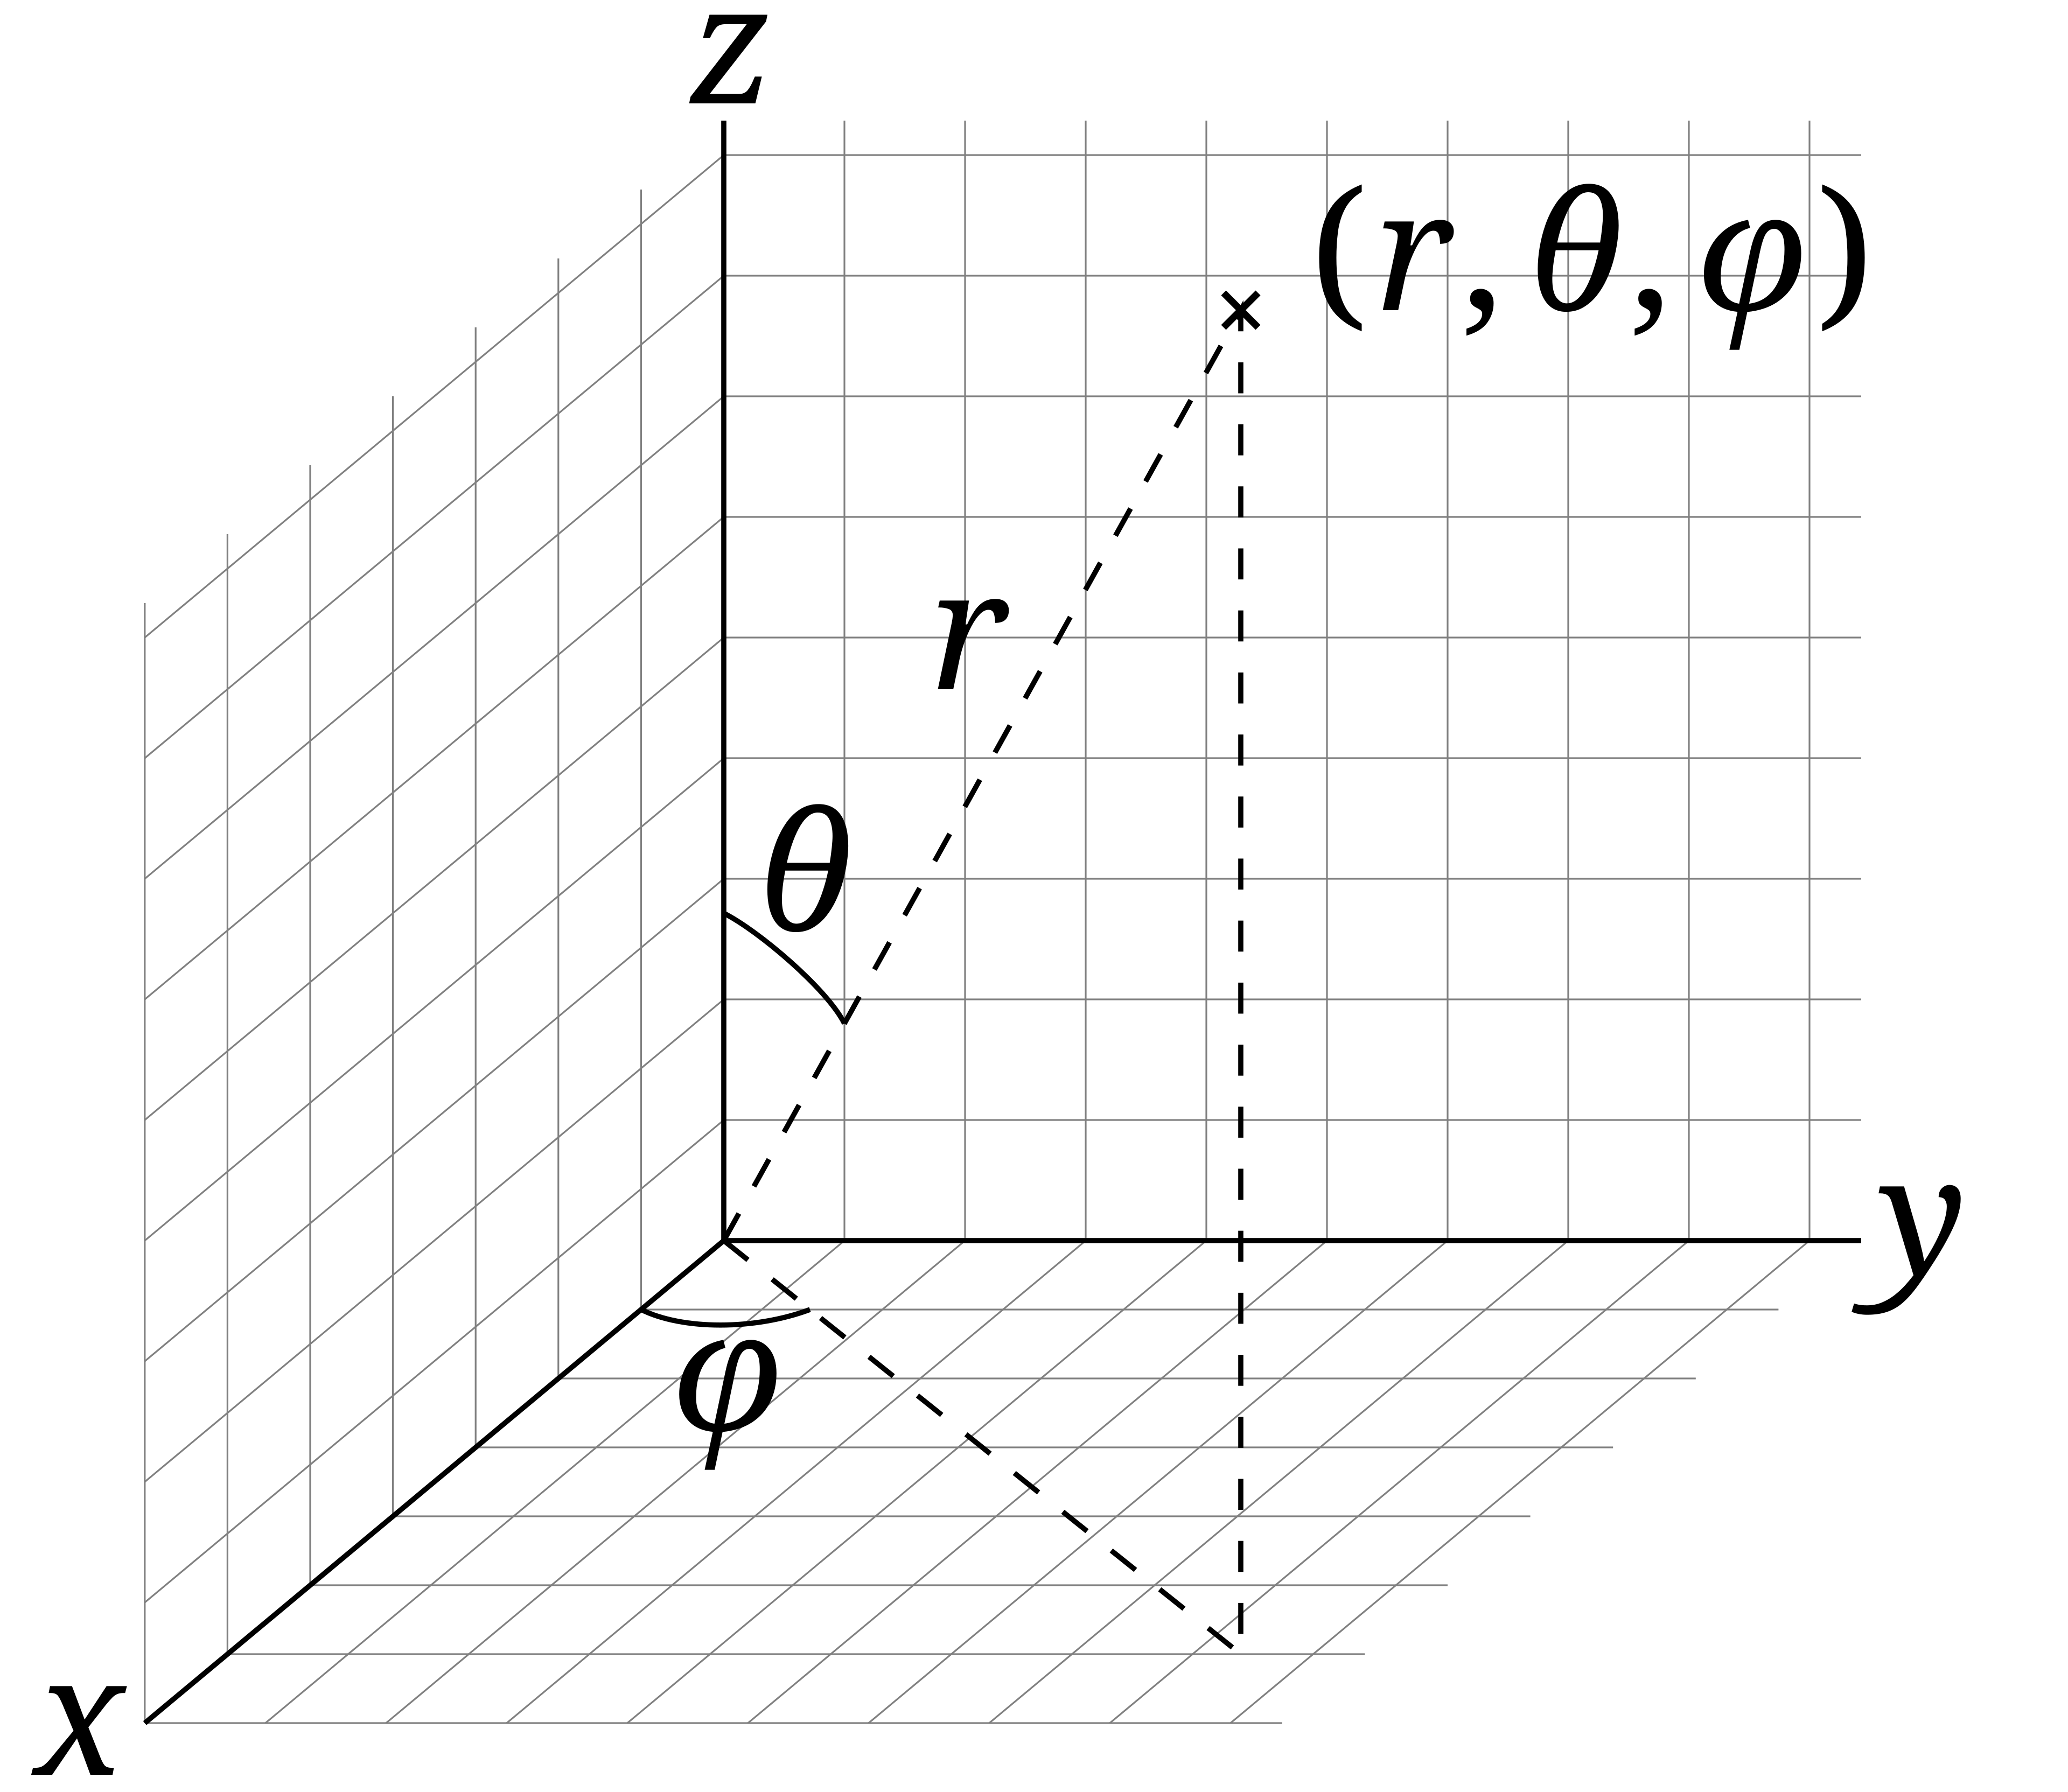
\includegraphics[width=0.5\linewidth]{3D_Spherical.png}
    \caption{Schematic description of spherical polar coordinates.}
    \label{fig:3D_spherical}
\end{figure}
Equation \eqref{eq:relEOM} splits into radial and tangential parts:
\begin{align}
\mu\big(\ddot r-r\dot\phi^2\big) &= -\nabla V(r), \label{eq:radial}\\
\mu\big(2\dot r\dot\phi+r\ddot\phi\big) &= 0\implies \dv{(r^2\dot{\phi})}{t}=0. \label{eq:tangential}
\end{align}
This was supposed to be a coupled differential equation. But because of equation \eqref{eq:tangential} is just angular momentum conservation, i.e. Kepler's second law again, since $\vecL=\mu\vecr\times\dot{\vecr}=\mu r^2\dot\phi\,\hat L$. So
\begin{equation}
\dot\phi = \frac{L}{\mu r^2}, \label{eq:phidot}
\end{equation}
and \eqref{eq:radial} becomes, eliminating $\dot\phi$,
\begin{equation}
\mu\ddot r - \frac{L^2}{\mu r^3} = -\nabla V(r). \label{eq:radial_reduced}
\end{equation}

\section{The Orbit Equation}

To get the orbit \emph{shape} $r(\phi)$ we change independent variable from $t$ to $\phi$ using \eqref{eq:phidot}: $\dfrac{dr}{dt}=\dot\phi\dfrac{dr}{d\phi}=\dfrac{L}{\mu r^2}\dfrac{dr}{d\phi}$, and
\[
\frac{d^2r}{dt^2}=\frac{L}{\mu r^2}\frac{d}{d\phi}\!\left[\frac{L}{\mu r^2}\frac{dr}{d\phi}\right]
=\frac{L^2}{\mu^2 r^4}\left[\frac{d^2r}{d\phi^2}-\frac{2}{r}\left(\frac{dr}{d\phi}\right)^2\right].
\]
Substituting into \eqref{eq:radial_reduced} and dividing by $L^2/(\mu r^4)$:
\[
\frac{1}{r^4}\left[\frac{d^2r}{d\phi^2}-\frac{2}{r}\left(\frac{dr}{d\phi}\right)^2\right]-\frac{1}{r^3}=-\frac{\mu}{L^2}\nabla V(r).
\]
The standard trick is the \textbf{Binet substitution} $r=1/\rho$: then $dr/d\phi=-\rho^{-2}d\rho/d\phi$ and $d^2r/d\phi^2=-\rho^{-2}d^2\rho/d\phi^2+2\rho^{-3}(d\rho/d\phi)^2$. Substituting and simplifying (the $(d\rho/d\phi)^2$ terms cancel), one obtains the \textbf{orbit equation}:
\begin{equation}
\boxed{\frac{d^2\rho}{d\phi^2}+\rho = \frac{\mu}{L^2}\frac{1}{\rho^2}\nabla V\!\left(\frac1\rho\right).} \label{eq:orbiteq}
\end{equation}
This is a purely geometric ODE for the orbit's shape, valid for any central potential.

\section{Keplerian Orbits}

For Newtonian gravity, $V(r)=-GM\mu/r$, so $\nabla V(r) = GM\mu\rho^2\,\rhat$. Equation \eqref{eq:orbiteq} becomes
\[
\frac{d^2\rho}{d\phi^2}+\rho =\frac{GM\mu^2}{L^2}.
\]

Shifting $\tilde\rho=\rho-GM\mu^2/L^2$ turns this into the simple-harmonic-oscillator equation $\ddot{\tilde\rho}+\tilde\rho=0$ (derivatives in $\phi$), with solution $\tilde\rho=A\cos(\phi-\omega)$ for constants $A,\omega$. In terms of $r=1/\rho$:
\[
r(\phi)=\left(\frac{GM\mu^2}{L^2}+A\cos(\phi-\omega)\right)^{-1}
=\frac{L^2/(GM\mu^2)}{1+\dfrac{L^2A}{GM\mu^2}\cos(\phi-\omega)}.
\]
Defining the \textbf{semi-latus rectum} $\lambda \equiv L^2/(GM\mu^2)$ as the value of $r$ when $\phi=\omega+90^{\circ}$ and \textbf{eccentricity} $e\equiv \lambda A$,
\begin{equation}
\boxed{r(\phi) = \frac{\lambda}{1+e\cos(\phi-\omega)}.} \label{eq:conic}
\end{equation}
This is the polar equation of a conic section with one focus at the origin, semi-latus rectum $\lambda$, eccentricity $e$, and major axis rotated by $\omega$ (the \textbf{argument of periapsis} — periapsis occurs at $\phi=\omega$). 
	\begin{figure}[H]
		\centering
		
		
		\usetikzlibrary{calc} %allows coordinate calculations
		
		% Newcommand
		
		%% Midline Label
		\newcommand{\midlinelabel}[3]{
			\node (midlabel) at ($ (#1)!.5!(#2) $) {#3};
			\draw[stealth-] (#1) --  (midlabel);
			\draw[-stealth] (midlabel) -- (#2);
		}
		%
		\newcommand{\midlinelabell}[3]{
			\node[fill = white, inner sep = 0.2pt, outer sep=3pt] (midlabel) at ($ (#1)!.5!(#2) $) {#3};
			\draw[stealth-] (#1) --  (midlabel);
			\draw[-stealth] (midlabel) -- (#2);
		}
		\newcommand{\midlinelabelll}[3]{
			\node[fill = white, inner sep = 0.2pt, outer sep=3pt,scale=0.6] (midlabel) at ($ (#1)!.5!(#2) $) {#3};
			\draw[stealth-] (#1) --  (midlabel);
			\draw[-stealth] (midlabel) -- (#2);
		}\usetikzlibrary{calc}
		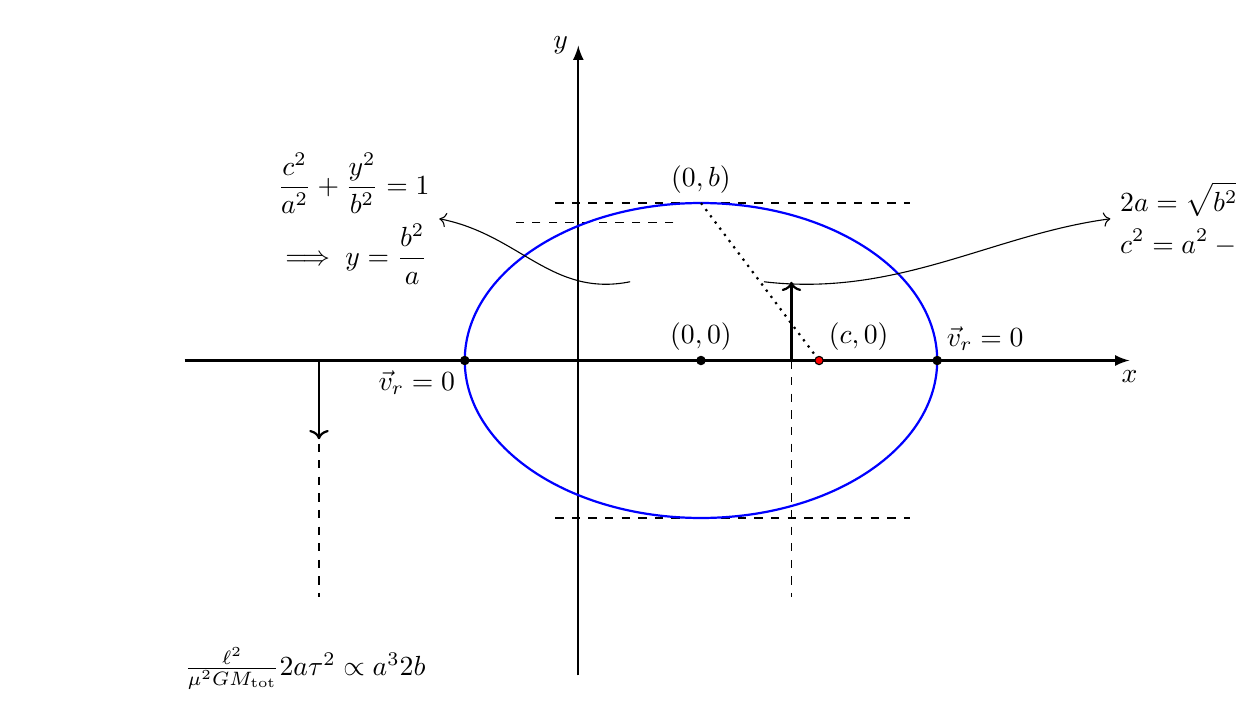
\begin{tikzpicture}
			% Axis
			\draw[-latex, thick] (5,0) -- (5,8) node[left] {$y$};
			\draw[-latex, thick] (0,4) -- (12,4) node[below] {$x$};
			\midlinelabell{3,4}{3,5.75}{$\frac{\ell^2}{\mu^2GM_{\rm tot}}$};
			
			% Key points
			\coordinate (F) at (5,4);       % illustrative focus = (c,0)
			\coordinate (Top) at (3.5,6);   % illustrative top point = (0,b)
			
			% Lines
			\draw[dashed] (5,5.75) -- (3,5.75);
			\draw[dashed] (0.5,4) -- (0.5,1);
			\draw[dashed] (6.5,4) -- (6.5,1);
			\draw[->,thick] (6.5,4)--(6.5,5);
			\draw[->,thick] (0.5,4)--(0.5,3);
			\draw[dashed] (3.5,2) -- (8,2);
			\draw[dashed] (3.5,6) -- (8,6);
			
			%% Labels
			\midlinelabel{0.5,1}{6.5,1}{$2a$}
			\midlinelabelll{3.5,3.5}{6.5,3.5}{$\tau^2\propto a^3$}
			\midlinelabell{8,2}{8,6}{$2b$}
			\midlinelabelll{6.5,7}{5,7}{perigee}
			\midlinelabelll{0.5,7}{5,7}{apogee}
			
			% Ellipse
			\draw[blue, thick] (3.5,4) circle [x radius = 3, y radius = 2];
			
			% Dotted line from (0,b) to (c,0)
			\draw[dotted, thick] (Top) -- (F);
			
			% Points
			\draw[fill=black] (3.5,4) circle [radius=1.5pt] node[above] {$(0,0)$};
			\draw[fill=black] (0.5,4) circle [radius=1.5pt] node[below left] {$\vec{v}_{r}=0$};
			\draw[fill=black] (6.5,4) circle [radius=1.5pt] node[above right] {$\vec{v}_{r}=0$};
			\draw[fill=red] (F) circle [radius=1.5pt] node[above right] {$(c,0)$};
			\node[above] at (Top)  {$(0,b)$};
			
			% Calculation on right
			\node[anchor=west, align=left] (calcbox) at (8.7,5.8) {
				$\displaystyle 2a=\sqrt{b^2+c^2}+\sqrt{b^2+c^2}$ \\[3pt]
				$\displaystyle c^2=a^2-b^2=a^2e^2$
			};
			\node[anchor=west, align=left] (calcbox2) at (-2,5.8) {
				$\displaystyle \frac{c^2}{a^2}+\frac{y^2}{b^2}=1$ \\[3pt]
				$\displaystyle \implies y=\frac{b^2}{a}$ 
			};
			% Squiggly arrow from focus to calculation
		\draw[->, thin]
		(4.3,5).. controls (6.0,4.8) and (7.2,5.6) ..
		(calcbox.west);
		\draw[->, thin]
		(2.6,5).. controls (1.6,4.8) and (1.2,5.6) ..
		(calcbox2.east);
		\end{tikzpicture}
	\end{figure}
Two more shape parameters follow:
\[
a=\frac{\lambda}{1-e^2}\ \text{(semi-major axis)}, \qquad b = a\sqrt{1-e^2}\ \text{(semi-minor axis)}.
\]
One can check this directly from the equation of the ellipse,
\begin{align}
\frac{x^2}{a^2}+\frac{y^2}{b^2} &= 1,
\end{align}
by writing the polar coordinates about the focus as
\begin{align}
x &= ae+r(\phi)\cos\phi,\\
y &= r(\phi)\sin\phi.
\end{align}
Substitution gives
\begin{align}
\frac{(ae+r\cos\phi)^2}{a^2}+\frac{r^2\sin^2\phi}{a^2(1-e^2)}&=1.
\end{align}
Solving for \(r\) then yields
\begin{align}
r(\phi)&=\frac{a(1-e^2)}{1+e\cos\phi}.
\end{align}

\begin{center}
\begin{tabular}{@{}ll@{}}
\toprule
Eccentricity & Conic section\\
\midrule
$e=0$ & circle\\
$0<e<1$ & ellipse ($E<0$, bound)\\
$e=1$ & parabola ($E=0$)\\
$e>1$ & hyperbola ($E>0$, unbound)\\
\bottomrule
\end{tabular}
\end{center}
Bound, closed elliptical orbits ($E<0$) constitute \textbf{Kepler's first law}. In the original (unreduced) frame,
\[
\vecx_1=\frac{m_2}{M}\vecr,\qquad \vecx_2=-\frac{m_1}{M}\vecr.
\]

\section{Energy and Angular Momentum in Terms of \texorpdfstring{$a,e$}{a,e}}

\subsection{Energy}
\[
E=\frac12\mu\dot{\vecr}^2-\frac{GM\mu}{r} = \frac12\mu\big(\dot r^2+r^2\dot\phi^2\big)-\frac{GM\mu}{r}
=\frac12\mu\dot r^2+\frac{L^2}{2\mu r^2}-\frac{GM\mu}{r}.
\]
Since $E$ is conserved, evaluate at periapsis ($\phi=\omega$), where $r=a-ae=\lambda/(1+e)$ and $\dot r=0$ (turning point of $r$):
\[
E = 0+\frac{L^2(1+e)^2}{2\mu\lambda^2}-\frac{GM\mu(1+e)}{\lambda}
=\frac{GM\mu^2\lambda(1+e)^2}{2\mu\lambda^2}-\frac{GM\mu(1+e)}{\lambda}
=-\frac{GM\mu}{2\lambda}(1-e^2),
\]
using $L^2=GM\mu^2\lambda$ (below). With $a=\lambda/(1-e^2)$,
\begin{equation}
\boxed{E=-\frac{GM\mu}{2a}.} \label{eq:visviva_E}
\end{equation}
Since $\lambda>0$ always, the sign of $E$ tracks $e$: bound orbits ($E<0$) have $e<1,\ a>0$; unbound orbits ($E\geq0$) have $e\geq1$; hyperbolic orbits formally have $a<0$.

\subsection{Angular momentum}
Both at apoapsis $(r=a+ae=\frac{\lambda}{1-e})$ and periapsis$(r=a-ae=\frac{\lambda}{1+e})$, we have $\dot{r}=0$,
\begin{align}
\frac{L^2(1+e)^2}{2\mu\lambda^2}-\frac{GM\mu(1+e)}{\lambda}
=\frac{L^2(1-e)^2}{2\mu\lambda^2}-\frac{GM\mu(1-e)}{\lambda}
\end{align}
Solving for $L$:
\begin{equation}
L=\sqrt{GM\mu^2\lambda}, \qquad\text{i.e.}\qquad L^2=GM\mu^2 a(1-e^2), \label{eq:L_of_ae}
\end{equation}
and, using \eqref{eq:Lhat},
\[
\vecL = \sqrt{GM\mu^2\lambda}\,\big(-\sin\Omega\sin\iota\,\hat\alpha+\cos\Omega\sin\iota\,\hat\delta+\cos\iota\,\hat R\big).
\]

\subsection{Instantaneous kinetic energy}
From $E=K+V$: $K=\tfrac12\mu\dot{\vecr}^2 = E-V= GM\mu\left(\dfrac1r-\dfrac1{2a}\right)$ — the \emph{vis-viva} equation. Splitting between the two bodies via $\vecx_i$: $K_1=\tfrac12 m_1v_1^2=\tfrac{m_2}{M}K$, $K_2=\tfrac{m_1}{M}K$.

\paragraph{Inverting for $a,e$.} Equations \eqref{eq:visviva_E}--\eqref{eq:L_of_ae} give the orbital elements directly from the (conserved) energy and angular momentum:
\begin{equation}
a=-\frac{GM\mu}{2E},\qquad e=\sqrt{1+\frac{2EL^2}{(GM)^2\mu^3}}. \label{eq:a_e_from_EL}
\end{equation}

\section{True and Eccentric Anomaly; Kepler's Equation}

We now want $r(t)$ (and hence $\phi(t)$), not just $r(\phi)$. From the vis-viva relation,
\[
\dot r = \sqrt{\frac{2}{\mu}\left(E-\frac{L^2}{2\mu r^2}+\frac{GM\mu}{r}\right)}
=\sqrt{GM}\,\frac1r\left(2r-\frac{r^2}{a}-\lambda\right)^{1/2},
\]
using \eqref{eq:visviva_E}--\eqref{eq:L_of_ae} to trade $E,L$ for $a,\lambda$. Then
\[
t-t_0 = \frac{1}{\sqrt{GM}}\int_{r_0}^{r}\frac{r'\,dr'}{\left(2r'-r'^2/a-\lambda\right)^{1/2}}.
\]

\subsection{Elliptical orbits: eccentric anomaly}
For $a>0$, substitute
\begin{equation}
r=a\big(1-e\cos u\big), \label{eq:r_of_u}
\end{equation}
where $u$ is the \textbf{eccentric anomaly} (this choice guarantees $r>0$ throughout, since $-1\le\cos u\le1$). Then $dr=ae\sin u\,du$, and the bracket under the square root simplifies (using $\lambda=a(1-e^2)$) to $a e^2\sin^2u$, so the square root is simply $\sqrt a\, e\,|\sin u|$. The integral collapses to
\[
t-t_0=\frac{a^{3/2}}{\sqrt{GM}}\int_0^u (1-e\cos u')\,du' = \frac{a^{3/2}}{\sqrt{GM}}\big[u-e\sin u\big],
\]
where $t_0$ (\textbf{epoch}) is the time at which $u=0$ — the sixth and final constant of integration, $T_0$.

\paragraph{Relating true anomaly $v$ and eccentric anomaly $u$:}
Define the \textbf{true anomaly} $v\equiv\phi-\omega$ (so $r=\lambda/(1+e\cos v)$ from \eqref{eq:conic}). Equating this with \eqref{eq:r_of_u}:
\[
\frac{1-e\cos u}{1-e^2}=\frac{1}{1+e\cos v}
\quad\Longrightarrow\quad
\cos v = \frac{\cos u - e}{1-e\cos u}. \tag{65a}
\]
Consistently,
\begin{equation}
\sin v = \frac{\sqrt{1-e^2}\sin u}{1-e\cos u},\qquad
\tan v = \frac{\sqrt{1-e^2}\sin u}{\cos u - e},\qquad
\tan\frac v2 = \sqrt{\frac{1+e}{1-e}}\,\tan\frac u2. \label{eq:v_of_u}
\end{equation}
At $u=0$ and $u=\pi$, $v=u$ — periapsis and apoapsis coincide for the two anomalies, as they must by symmetry.

\subsection{Hyperbolic trajectories}
For $a<0$ (and $e>1$), the analogous substitution is $r=a(1-e\cosh u)$ (using $\cosh u\ge1$ keeps $r>0$ since $a<0$). Carrying through the same integral gives the \textbf{hyperbolic} anomaly relation
\[
t-t_0 = \frac{(-a)^{3/2}}{\sqrt{GM}}\big[e\sinh u - u\big],
\]
with true-anomaly relations
\begin{equation}
\cos v = \frac{e-\cosh u}{e\cosh u - 1},\qquad
\sin v = \frac{\sqrt{e^2-1}\sinh u}{e\cosh u-1},\qquad
\tan\frac v2=\sqrt{\frac{e+1}{e-1}}\tanh\frac u2. \label{eq:v_of_u_hyp}
\end{equation}

\section{Kepler's Third Law}

For one complete orbit, $u$ advances by $2\pi$ while $t$ advances by the orbital period $2\pi/n$ ($n\equiv$ mean motion):
\begin{equation}
\frac{2\pi}{n} = \frac{a^{3/2}}{\sqrt{GM}}\big[2\pi - e\sin(2\pi)\big] = \frac{a^{3/2}}{\sqrt{GM}}\cdot2\pi
\quad\Longrightarrow\quad
\boxed{n=\sqrt{\frac{GM}{a^3}},\qquad n^2a^3=GM.} \label{eq:kepler3}
\end{equation}

\section{Kepler's Equation}

Substituting $n=\sqrt{GM/a^3}$ into $t-t_0=(a^{3/2}/\sqrt{GM})(u-e\sin u)$ and defining the \textbf{mean anomaly} $\ell\equiv n(t-t_0)$:
\begin{equation}
\boxed{\ell = u - e\sin u} \qquad\text{(elliptical Kepler's equation).} \label{eq:kepler_eq}
\end{equation}
This transcendental equation must be solved numerically (or by series, \S\ref{sec:bessel}) for $u(\ell)$, i.e.\ $u(t)$. The hyperbolic analogue (with $n\equiv GM/(-a)^{3/2}$) is
\begin{equation}
\ell = e\sinh u - u. \label{eq:kepler_eq_hyp}
\end{equation}

\section{Keplerian Parametrization}
\label{sec:parametrization}

\subsection{Elliptical orbits}
Collecting results:
\begin{align}
r&=a(1-e\cos u), & \phi&=v+\omega,\\
\tan\frac v2 &= \sqrt{\frac{1-e}{1+e}}\tan\frac u2, & \ell&=u-e\sin u.
\end{align}

Differentiating Kepler's equation \eqref{eq:kepler_eq} in $t$: $n=\dot u(1-e\cos u)$, so
\begin{equation}
\dot u = \frac{n}{1-e\cos u}. \label{eq:udot}
\end{equation}
Differentiating $r=a(1-e\cos u)$:
\begin{equation}
\dot r = ae\sin u\,\dot u = \frac{an\,e\sin u}{1-e\cos u}. \label{eq:rdot_u}
\end{equation}
Differentiating the $v$-$u$ relation and using \eqref{eq:v_of_u}, one finds $dv/du = \sqrt{1-e^2}/(1-e\cos u)$, so
\begin{equation}
\dot\phi = \dot v = \frac{dv}{du}\dot u = \frac{n\sqrt{1-e^2}}{(1-e\cos u)^2}. \label{eq:phidot_u}
\end{equation}

\subsection{Hyperbolic trajectories}
Analogously, with $r=-a(e\cosh u - 1)$, $\phi=v+\omega$, $\tan(v/2)=\sqrt{(e+1)/(e-1)}\tanh(u/2)$, $\ell=e\sinh u - u$:
\begin{equation}
\dot u = \frac{n}{e\cosh u - 1},\quad
\dot r = -an\,\frac{e\sinh u}{e\cosh u - 1},\quad
\dot\phi=\dot v = \frac{n\sqrt{e^2-1}}{(e\cosh u-1)^2}. \label{eq:hyp_derivs}
\end{equation}

\section{Hyperbolic-Trajectory Parameters}

For unbound ($e>1$) encounters, four derived quantities are standard:

\textbf{Hyperbolic excess velocity} $v_\infty$: from $\tfrac12\mu\dot{\vecr}_\infty^2 = -GM\mu/(2a)$ (recall $a<0$),
\begin{equation}
|\dot{\vecr}_\infty| = \sqrt{-\frac{GM}{a}}. \label{eq:vinf}
\end{equation}

\textbf{Scattering angle} $\theta_\infty$: half the angle between the two asymptotes,
\begin{equation}
\cos\theta_\infty = -\lim_{u\to\infty}\frac{e-\cosh u}{e\cosh u -1} = \frac1e. \label{eq:scattering}
\end{equation}

\textbf{Periapsis distance}:
\begin{equation}
r_p = \min_v \frac{a(1-e^2)}{1+e\cos v} = -a(e-1). \label{eq:rp}
\end{equation}

\textbf{Semi-minor axis / impact parameter}: the semi-minor axis $b=-a\sqrt{e^2-1}$ satisfies $-ab=\lambda$. The impact parameter $b'$ (miss distance of the unperturbed asymptote) is
\[
b' = (-a+r_p)\sin\theta_\infty = -ae\sin\theta_\infty = -a\sqrt{e^2-1} = b,
\]
i.e.\ impact parameter and semi-minor axis coincide.

\textbf{Flight-path angle} (angle between $\dot{\vecr}$ and the direction $\perp\rhat$ in-plane):
\begin{equation}
\sin\varphi = \frac{\dot{\vecr}\cdot\rhat}{|\dot{\vecr}|}=\frac{\dot r}{\sqrt{\dot r^2+r^2\dot\phi^2}}. \label{eq:flightpath}
\end{equation}

\section{Fourier Solution of Kepler's Equation}
\label{sec:bessel}

Kepler's equation $u-\ell=e\sin u$ can be solved as a Fourier series in $\ell$:
\[
e\sin u = \sum_{s=1}^{\infty}A_s\sin(s\ell).
\]
Using $A_s = \tfrac2\pi\int_0^\pi (u-\ell)\sin(s\ell)\,d\ell$, integrating by parts (the boundary term vanishes since $u=\ell$ at $\ell=0,\pi$), and substituting $d\ell = (1-e\cos u)\,du$ (from Kepler's equation) turns the $\ell$-integral into a $u$-integral:
\[
A_s = \frac{2}{s\pi}\int_0^\pi \cos(su-se\sin u)\,du = \frac{2}{s}J_s(se),
\]
recognizing the integral representation of the Bessel function of the first kind, $J_s(x)=\tfrac1\pi\int_0^\pi\cos(s\tau-x\sin\tau)\,d\tau$. So
\begin{equation}
u(\ell) = \ell + \sum_{s=1}^{\infty}\frac{2}{s}J_s(se)\sin(s\ell). \label{eq:kepler_series}
\end{equation}
This is the classical Bessel-function series solution to Kepler's equation.

\section{The Laplace--Runge--Lenz Vector}

Define $\vecA \equiv \vecp\times\vecL - GM\mu^2\rhat$ (with $\vecp=\mu\dot{\vecr}$). For the pure Kepler problem,
\[
\dot{\vecA} = \dot{\vecp}\times\vecL - GM\mu^2\dot{\rhat}
= -\frac{GM\mu}{r^2}\big(\rhat\times\vecL\big) - GM\mu^2\dot\phi\,\phihat.
\]
Using $\vecL=L\hat L$, planar motion identities $\rhat\times\hat L=-\phihat$, and $\dot\phi=L/(\mu r^2)$ from \eqref{eq:phidot}:
\[
\dot{\vecA} = -GM\mu\left(\frac{L}{r^2}\phihat - \mu\dot\phi\,\phihat\right)=0,
\]
so $\vecA$ is conserved for the unperturbed problem — it is a \emph{fourth}, non-obvious constant of the Kepler problem (beyond $E,\vecL$), reflecting the extra "hidden" $SO(4)$ symmetry of the $1/r$ potential.

\paragraph{Direction and magnitude of $\vecA$.} From the definition it is clear that $\vecA$ is planar. Therefore, we can decompose it as $\vecA=A_r\hat{r}+A_{\phi}\hat{\phi}$.

\begin{figure}[H]
	\centering
	\tdplotsetmaincoords{70}{115}
	
	\begin{tikzpicture}[
		tdplot_main_coords,
		scale=1.5,
		>=stealth
		]
		
		%------------------------------------------------
		% Parameters
		%------------------------------------------------
		
		\def\a{2.8}
		\def\e{0.45}
		
		\pgfmathsetmacro{\b}{\a*sqrt(1-\e*\e)}
		\pgfmathsetmacro{\ae}{\a*\e}
		\pgfmathsetmacro{\rp}{-\a*(1-\e)}
		
		%------------------------------------------------
		% Orbital plane
		%------------------------------------------------
		
		\fill[gray!10]
		(-3.2,-3.3,0)
		-- (5.2,-3.3,0)
		-- (5.2,3.3,0)
		-- (-3.2,3.3,0)
		-- cycle;
		
		\draw[gray!40]
		(-3.2,-3.3,0)
		-- (5.2,-3.3,0)
		-- (5.2,3.3,0)
		-- (-3.2,3.3,0)
		-- cycle;
		
		%------------------------------------------------
		% Coordinate axes
		%------------------------------------------------
		
		\draw[->,thin]
		(4.1,0,0)--(-3.1,0,0) 
		node[left] {$x$};
		
		\draw[->,thin]
		(0,2.1,0)--(0,-2.1,0)
		node[above] {$y$};
		
		\draw[->,thin]
		(0,0,0) -- (0,0,1.8)
		node[above] {$z$};
		
		%------------------------------------------------
		% Ellipse
		%------------------------------------------------
		
		\draw[thick]
		plot[
		variable=\theta,
		domain=0:360,
		samples=150
		]
		(
		{\ae+\a*cos(\theta)},
		{\b*sin(\theta)},
		{0}
		);
		
		%------------------------------------------------
		% Focus
		%------------------------------------------------
		
		\fill (0,0,0) circle (0.04);
		\node[below right] at (0,0,0) {$F$};
		
		%------------------------------------------------
		% Perigee
		%------------------------------------------------
		
		\fill (\rp,0,0) circle (0.045);\node[below right] at (\rp,0,0) {$P$};
		
		%------------------------------------------------
		% r-hat: Focus -> Perigee
		%------------------------------------------------
		
		\draw[->,very thick]
		(0,0,0)	-- (\rp,0,0)node[midway,above] {$\hat{\mathbf r}$};
		
		%------------------------------------------------
		% p-hat: tangent at Perigee
		%------------------------------------------------
		
		\draw[->,very thick]
		(\rp,0,0)--(\rp,-1.35,0)
		node[above right] {$\hat{\mathbf p}$};
		
		%------------------------------------------------
		% L-hat: normal to orbital plane at Perigee
		%------------------------------------------------
		
		\draw[->,very thick]
		(\rp,0,0)
		-- (\rp,0,1.35)
		node[right] {$\hat{\mathbf L}$};
		
		%------------------------------------------------
		% Relation
		%------------------------------------------------
		
		\node at (2.0,1.8,0.25)
		{$\hat{\mathbf p}\times\hat{\mathbf L}
			=\hat{\mathbf r}$};
		
	\end{tikzpicture}
	\caption{The Runge Lenz vector points radially outward at perigee. Since it is conserved, the direction and magnitude stays fixed during the entire evolution.}
\end{figure}
At periapsis the velocity is purely tangential ($\vecp\perp\rhat$), so $\rhat\times\vecA\big|_{\rm peri}=\rhat\times(\vecp\times\vecL)\big|_{\rm peri}=\big[\vecp(\rhat\cdot\vecL)-\vecL(\rhat\cdot\vecp)\big]_{\rm peri}=0$ (both dot products vanish there). Also $\rhat\cdot\vecA|_{\rm peri}=A$ (from the relation above with $v=0$ at periapsis). Together these mean $\hat A = \rhat|_{\rm peri}$: $\vecA$ points from the focus \emph{towards periapsis}.

Since $\vecA$ points radially outwards at the Periapsis. We find the magnitude by doting $\vecA$ into $\vecr$:
\begin{align}
    \vecA\cdot\vecr &= (\vecp\times\vecL)\cdot\vecr - GM\mu^2 r \\
    &=p_i L_j \epsilon_{ijk}r_k-GM\mu^2 r=p_i L_j \epsilon_{kij}r_k-GM\mu^2 r\\
    &= \underbrace{(\vecr\times\vecp)}_{\vecL}\cdot\vecL - GM\mu^2 r = L^2 - GM\mu^2 r,\end{align}
i.e., writing $\vecA\cdot\vecr = Ar\cos v$ (with $v$ the angle between $\vecA$ and $\vecr$), using
\[
r = \frac{L^2/(GM\mu^2)}{1+e\cos v}\implies GM\mu^2 r = \frac{L^2}{1+e\cos v}.
\]
We find:
\begin{align}
	Ar\cos v&=L^2 - GM\mu^2 r,\\
	A \frac{L^2/GM\mu^2}{1+e\cos v}\cos v&=L^2\left(1-\frac{1}{1+e\cos v}\right)=\frac{L^2e\cos v}{1+e\cos v}
\end{align}

Hence
\begin{equation}
\boxed{A = GM\mu^2 e.} \label{eq:A_magnitude}
\end{equation}
Using \eqref{eq:rhat_phihat}:
\begin{equation}
\hat A = \cos\omega\,\hatn+\sin\omega\,\hat y. \label{eq:Ahat}
\end{equation}
Equivalently, the \textbf{eccentricity vector} $\vec e \equiv \vecA/(GM\mu^2) = e\hat A$ is a conserved vector encoding $(e,\omega)$ together. Since $e,\Omega,\iota$ are already determined by $(E,\vecL)$, the only \emph{new} information in $\vecA$ is $\omega$ — the in-plane orientation of the ellipse.

\section{Perturbed Orbits}

Now add a perturbing force $\vecF$ (not necessarily central) to the Kepler problem:
\begin{equation}
\mu\ddot{\vecr}+\frac{GM\mu}{r^2}\rhat = \vecF. \label{eq:perturbed_eom}
\end{equation}

\subsection{The osculating-orbit ansatz (variation of parameters)}
\label{sec:osculating_ansatz}

Before writing down rates for $a,e,\iota,\Omega,\omega$, it is worth being explicit about \emph{why} this is a sensible thing to do at all — this justification was skipped in the reference notes but is worth reconstructing, since it is what turns "$a$" from a constant of the unperturbed problem into a well-defined, instantaneously-meaningful function $a(t)$ of the perturbed one.

For the unperturbed ($\vecF=0$) problem, the solution is fully determined by six constants $Q_i\ (i=1,\dots,6)$ — take these to be $(a,e,\iota,\Omega,\omega,T_0)$ — through fixed functional forms
\[
\vecr = \vecr(Q_1,\dots,Q_6,t), \qquad \dot{\vecr}=\dot{\vecr}(Q_1,\dots,Q_6,t)
\]
(these are exactly the formulas of \S\ref{sec:parametrization} translated into Cartesian orbital-plane components via \eqref{eq:rhat_phihat}). With $\vecF\neq0$ the true trajectory is no longer a fixed ellipse, but at every instant it is tangent to \emph{some} ellipse. The \textbf{osculating-orbit ansatz} keeps the same functional forms but promotes $Q_i\to Q_i(t)$, and \emph{defines} the instantaneous ellipse by requiring that the true velocity still be given by the same function $\dot{\vecr}(Q_i,t)$ that described the unperturbed problem — i.e., that position and velocity are simultaneously matched to some instantaneous Kepler orbit, not just position alone.

Concretely: differentiating $\vecr(Q_i(t),t)$,
\begin{equation}
\frac{d\vecr}{dt}=\left.\frac{\partial\vecr}{\partial t}\right|_{Q_i}+\sum_{i=1}^6\frac{\partial\vecr}{\partial Q_i}\frac{dQ_i}{dt}.
\end{equation}
By construction $\partial\vecr/\partial t|_{Q_i}=\dot{\vecr}(Q_i,t)$. Requiring the true velocity to equal this same function forces
\begin{equation}
\sum_{i=1}^{6}\frac{\partial\vecr}{\partial Q_i}\frac{dQ_i}{dt}=0. \label{eq:osculating_constraint}
\end{equation}
This is a vector equation ($3$ scalar constraints). It is a \emph{gauge choice}, not extra physics — it is exactly what makes the instantaneous ellipse "osculating" (tangent in both position and velocity), and it is always solvable for the $\dot Q_i$ alongside the equation below, so no generality is lost.

Differentiating $\dot{\vecr}(Q_i(t),t)$ similarly:
\[
\frac{d\dot{\vecr}}{dt}=\left.\frac{\partial\dot{\vecr}}{\partial t}\right|_{Q_i}+\sum_{i=1}^6\frac{\partial\dot{\vecr}}{\partial Q_i}\frac{dQ_i}{dt}.
\]
Since $\dot{\vecr}(Q_i,t)$ solves the \emph{unperturbed} problem for fixed $Q_i$, $\partial\dot{\vecr}/\partial t|_{Q_i}=-GM\rhat/r^2$. The left side is the true acceleration, given by \eqref{eq:perturbed_eom}. Equating and cancelling the common $-GM\rhat/r^2$:
\begin{equation}
\sum_{i=1}^{6}\frac{\partial\dot{\vecr}}{\partial Q_i}\frac{dQ_i}{dt}=\frac{\vecF}{\mu}. \label{eq:osculating_constraint2}
\end{equation}
Another vector equation, $3$ more scalar constraints. Together, \eqref{eq:osculating_constraint} and \eqref{eq:osculating_constraint2} give $3+3=6$ scalar equations for the $6$ unknowns $\dot Q_i$ — an exactly determined linear system (given the Jacobian relating $(\vecr,\dot{\vecr})$ to $(Q_i)$ is non-singular, true away from degenerate orbits such as $e=0$ or $\iota=0$). Solving this system for the $\dot Q_i$ is precisely what produces the Lagrange/Gauss planetary equations derived below — e.g.\ Eqs.~\eqref{eq:adot}, \eqref{eq:edot}, \eqref{eq:omegadot}, \eqref{eq:Ldot_pert}. The derivations of $\dot E,\dot{\vecL},\dot{\vecA}$ that follow are exact identities for the true trajectory and do not by themselves need this ansatz; what the ansatz supplies is the licence to \emph{read} $a(t)=-GM\mu/2E(t)$, etc., as the semi-major axis of a genuine instantaneous ellipse rather than just a convenient bookkeeping variable.

\subsection{Rates of the fundamental constants}

Repeating the conservation-law derivations of \S1.3 with the extra force:
\begin{align}
\dot E &= \dot{\vecr}\cdot\vecF, \label{eq:Edot_pert}\\
\dot{\vecL} &= \vecr\times\vecF, \label{eq:Ldot_pert}\\
\dot{\vecA} &= \vecF\times\vecL + \mu\dot{\vecr}\times(\vecr\times\vecF). \label{eq:Adot_pert_raw}
\end{align}
For \eqref{eq:Edot_pert}: the Kepler-force terms cancel exactly as in \S1.3 (that cancellation used nothing but $\vecF=0$ for those terms), leaving only the work done by $\vecF$. For \eqref{eq:Ldot_pert}: the Kepler-force contribution $\vecr\times(-GM\mu\rhat/r^2)$ vanishes identically since $\vecr\parallel\rhat$, leaving only the torque from $\vecF$. For $\dot{\vecA}$: since $\vecA$ is exactly conserved when $\vecF=0$, every term \emph{not} containing $\vecF$ in the full expansion must sum to zero (this is the same cancellation verified explicitly for the $\alpha/r^3$ example in \S\ref{sec:worked}), leaving
\[
\dot{\vecA} = \vecF\times\vecL + \mu\dot{\vecr}\times(\vecr\times\vecF).
\]
Expand the double cross product ($\vec a\times(\vec b\times\vec c)=\vec b(\vec a\cdot\vec c)-\vec c(\vec a\cdot\vec b)$):
\[
\mu\dot{\vecr}\times(\vecr\times\vecF) = \mu\vecr(\dot{\vecr}\cdot\vecF)-\mu\vecF(\dot{\vecr}\cdot\vecr) = \mu\vecr(\dot{\vecr}\cdot\vecF)-\mu r\dot r\,\vecF.
\]
Writing $\vecr=r\rhat$ and factoring $\mu r\dot r$:
\[
\dot{\vecA} = \vecF\times\vecL + \mu r\dot r\left[\frac{(\dot{\vecr}\cdot\vecF)}{\dot r}\rhat - \vecF\right].
\]
Using $r\dot r = L\,e\sin v/(GM\mu^2/L)\cdot(\ldots)$, i.e.\ converting $\mu r\dot r$ to $L$ times a function of $v$ via $r=\lambda/(1+e\cos v)$, $\dot r = (L e/(\mu\lambda))\sin v$ (from \S\ref{sec:worked}'s kinematics), gives the compact form
\begin{equation}
\dot{\vecA} = L\left[\vecF\times\hat L + \frac{e\sin v}{1+e\cos v}\left(\frac{(\dot{\vecr}\cdot\vecF)}{\dot r}\rhat-\vecF\right)\right]. \label{eq:Adot_pert_compact}
\end{equation}

\subsection{Special case: $\vecF$ in the orbital plane}

Write $\vecF=F_r\rhat+F_\phi\phihat$ (no out-of-plane component). Then:
\begin{align}
\dot E &= \dot r F_r + r\dot\phi F_\phi, \label{eq:Edot_planar}\\
\dot L &= rF_\phi, \qquad \dot{\hat L}=0. \label{eq:L_planar}
\end{align}
Since $\dot{\hat L}=0$, \textbf{the orbital plane does not precess}: $\dot\Omega=\dot\iota=0$ whenever the perturbation is confined to the orbital plane (no out-of-plane component) — this generalizes the exact statement we found for the purely radial example (there, $F_\phi=0$ too, but the plane-fixing only needed $F_z=0$).

Working through \eqref{eq:Adot_pert_compact} with $\vecF=F_r\rhat+F_\phi\phihat$ (using $\rhat\times\hat L=-\phihat$, $\phihat\times\hat L=\rhat$, and $r\dot\phi/\dot r = (1+e\cos v)/(e\sin v)\equiv 1/\xi$ with $\xi\equiv e\sin v/(1+e\cos v)$) gives, after simplification,
\begin{equation}
\dot{\vecA} = L\left[2F_\phi\,\rhat - \Big(F_r+\xi F_\phi\Big)\phihat\right]. \label{eq:Adot_planar}
\end{equation}

\paragraph{Rate of $|\vecA|$ (i.e.\ $\dot e$).} Projecting \eqref{eq:Adot_planar} onto $\hat A=\cos\omega\,\hatn+\sin\omega\,\hat y$ (using $\rhat\cdot\hat A=\cos v$, $\phihat\cdot\hat A=-\sin v$, since $v=\phi-\omega$):
\begin{equation}
\dot A \equiv \dot{\vecA}\cdot\hat A= L\Big[F_r\sin v + F_\phi\big(2\cos v+\xi\sin v\big)\Big]. \label{eq:Amagdot}
\end{equation}
(Since $A=GM\mu^2e$, this directly gives $\dot e = \dot A/(GM\mu^2)$.)

\paragraph{Rate of $\hat A$'s rotation (i.e.\ $\dot\omega$).} Subtracting off the magnitude-changing piece, $A\dot{\hat A} = \dot{\vecA}-\dot A\,\hat A$, and using $\hat A = \cos v\,\rhat-\sin v\,\phihat$ (which follows from $\hat A\cdot\rhat=\cos v$, $\hat A\cdot\phihat=-\sin v$ together with orthonormality) one finds, after simplification,
\begin{equation}
A\dot{\hat A} = -L\Big[F_r\cos v + F_\phi(\xi\cos v - 2\sin v)\Big]\big(\sin v\,\rhat+\cos v\,\phihat\big). \label{eq:Ahatdot}
\end{equation}
Since $\hat A$ rotates purely by $\omega$ changing (with $\Omega,\iota$ fixed), $\dot{\hat A}$ has magnitude $|\dot\omega|$ in the direction transverse to $\hat A$; carrying through the projection (this is the step where the reference notes work through dotting with $\hatn$ and dividing by $\sin\omega$ — algebra that is fiddly but standard) gives
\begin{equation}
\boxed{\dot\omega = -\frac1e\sqrt{\frac{a(1-e^2)}{GM\mu^2}}\Big[F_r\cos v+F_\phi\big(\xi\cos v - 2\sin v\big)\Big].} \label{eq:omegadot}
\end{equation}


\paragraph{Rate of $a$.} From $E=-GM\mu/(2a)\Rightarrow\dot a = (2a^2/GM\mu)\dot E$, and \eqref{eq:Edot_planar} with $\dot r = (Le/\mu\lambda)\sin v$, $r\dot\phi = L/(\mu r)=(L/\mu\lambda)(1+e\cos v)$:
\begin{equation}
\dot a = \sqrt{\frac{4a^3}{GM\mu^2(1-e^2)}}\Big[e\sin v\,F_r + (1+e\cos v)F_\phi\Big]. \label{eq:adot}
\end{equation}
\paragraph{Rate of $e$.} From \eqref{eq:Amagdot} and $A=GM\mu^2e$:
\begin{equation}
\dot e = \sqrt{\frac{a(1-e^2)}{GM\mu^2}}\Big[F_r\sin v + F_\phi\big(2\cos v+\xi\sin v\big)\Big]. \label{eq:edot}
\end{equation}

\paragraph{Rate of true anomaly.} From $\cos v = \hat A\cdot\rhat$ differentiated, and using $\dot\phi=L/(\mu r^2)$:
\begin{equation}
\dot v = \sqrt{\frac{GM}{a^3(1-e^2)^3}}\big(1+e\cos v\big)^2 - \dot\omega. \label{eq:vdot}
\end{equation}

\paragraph{Osculating-element summary (planar perturbation).}
\begin{align}
\dot a &= \sqrt{\frac{4a^3}{GM\mu^2(1-e^2)}}\Big[e\sin v\,F_r+(1+e\cos v)F_\phi\Big], \notag\\
\dot e &= \sqrt{\frac{a(1-e^2)}{GM\mu^2}}\Big[F_r\sin v+F_\phi(2\cos v+\xi\sin v)\Big], \notag\\
\dot\Omega &= 0,\qquad \dot\iota=0, \notag\\
\dot\omega &= -\frac1e\sqrt{\frac{a(1-e^2)}{GM\mu^2}}\Big[F_r\cos v + F_\phi(\xi\cos v-2\sin v)\Big], \notag\\
\dot v &= \sqrt{\frac{GM}{a^3(1-e^2)^3}}(1+e\cos v)^2 - \dot\omega. \notag
\end{align}

\subsection{Nearly circular orbits: Laplace--Lagrange variables}

As $e\to0$, $\omega$ becomes ill-defined (periapsis is not a meaningful point on a circle) and $\dot\omega$ formally diverges in \eqref{eq:omegadot}. The fix is to use the Cartesian components of $\vecA$ directly instead of its polar decomposition:
\begin{equation}
\epsilon_1 \equiv e\cos\omega = \frac{A_1}{GM\mu^2},\qquad \epsilon_2\equiv e\sin\omega=\frac{A_2}{GM\mu^2}, \label{eq:LL_vars}
\end{equation}
together with $\Phi\equiv\omega+\ell = n(t-T)$ ($T$ = time of ascending-node passage) in place of $v$. To $O(e)$, the orbit parametrization becomes
\begin{align}
r &= a\big(1-\epsilon_1\cos\Phi-\epsilon_2\sin\Phi\big), \label{eq:r_LL}\\
\phi &= \Phi + 2\epsilon_1\sin\Phi - 2\epsilon_2\cos\Phi, \label{eq:phi_LL}\\
\dot r &= \frac{L}{a\mu}\big(\epsilon_1\sin\Phi-\epsilon_2\cos\Phi\big), \label{eq:rdot_LL}\\
\dot\phi &= \frac{L}{a^2\mu}\big(1+2\epsilon_1\cos\Phi+2\epsilon_2\sin\Phi\big). \label{eq:phidot_LL}
\end{align}
Repeating the perturbation analysis with $\delta\phi\equiv\phi-\Phi=\epsilon_1\sin\Phi-\epsilon_2\cos\Phi$ (to leading order in $e$) gives the osculating equations in this basis:
\begin{align}
\dot a &= \sqrt{\frac{4a^3}{GM\mu^2}}\Big[\delta\phi\,F_r + (1+\epsilon_1\cos\Phi+\epsilon_2\sin\Phi)F_\phi\Big], \label{eq:adot_LL}\\
\dot\epsilon_1 &= \sqrt{\frac{a}{GM\mu^2}}\Big[\sin\Phi\,F_r+2\cos\Phi\,F_\phi+\delta\phi(2\cos\Phi\,F_r-3\sin\Phi\,F_\phi)\Big], \label{eq:eps1dot}\\
\dot\epsilon_2 &= \sqrt{\frac{a}{GM\mu^2}}\Big[-\cos\Phi\,F_r+2\sin\Phi\,F_\phi+\delta\phi(2\sin\Phi\,F_r+3\cos\Phi\,F_\phi)\Big], \label{eq:eps2dot}\\
\dot\iota&=0,\qquad \dot\Omega=0,\qquad
\dot\Phi = \sqrt{\frac{GM}{a^3}}+O(e^2). \label{eq:Phidot_LL}
\end{align}
Using $\Phi$ as the independent variable ($dt/d\Phi=\sqrt{a^3/GM}$) removes explicit time dependence:
\begin{align}
\frac{da}{d\Phi} &= \frac{2a^3}{GM\mu}\Big[\delta\phi\,F_r+(1+\epsilon_1\cos\Phi+\epsilon_2\sin\Phi)F_\phi\Big], \label{eq:dadPhi}\\
\frac{d\epsilon_1}{d\Phi} &= \frac{a^2}{GM\mu}\Big[\sin\Phi\,F_r+2\cos\Phi\,F_\phi+\delta\phi(2\cos\Phi\,F_r-3\sin\Phi\,F_\phi)\Big], \label{eq:deps1dPhi}\\
\frac{d\epsilon_2}{d\Phi} &= \frac{a^2}{GM\mu}\Big[-\cos\Phi\,F_r+2\sin\Phi\,F_\phi+\delta\phi(2\sin\Phi\,F_r+3\cos\Phi\,F_\phi)\Big]. \label{eq:deps2dPhi}
\end{align}

\section{Rømer Delay for a Keplerian Orbit}

For a signal emitted from the primary body, the light-travel-time (Rømer) delay from the changing distance to the barycentre is $\Delta_R = -\tfrac1c\vecx_1\cdot\hat R = -\tfrac1c\tfrac{m_2}{M}\vecr\cdot\hat R$. Using $\vecr=r(v)\big(\cos\phi\,\hatn+\sin\phi\,\hat y\big)$ and the definitions \eqref{eq:node}--\eqref{eq:yhat} of $\hatn,\hat y$ in terms of $\hat\alpha,\hat\delta,\hat R$, all terms proportional to $\hat\alpha\cdot\hat R,\hat\delta\cdot\hat R$ (which vanish by orthogonality) drop, leaving only the $\hat R\cdot\hat R=1$ piece:
\[
\Delta_R = \frac1c\frac{m_2}{M}r(v)\sin\phi\sin\iota = \frac1c\frac{m_2}{M}r(v)\sin(v+\omega)\sin\iota.
\]
Expanding $\sin(v+\omega)=\cos v\sin\omega+\sin v\cos\omega$ and substituting $r\cos v = a(\cos u - e)$, $r\sin v = a\sqrt{1-e^2}\sin u$ (from \eqref{eq:v_of_u} and $r=a(1-e\cos u)$):
\begin{equation}
\Delta_R = \frac{a_1\sin\iota}{c}\Big[(\cos u - e)\sin\omega+\sqrt{1-e^2}\sin u\cos\omega\Big], \qquad a_1\equiv \frac{m_2}{M}a. \label{eq:romer}
\end{equation}

\section{Worked Example: the Radial Perturbation $\vecF=\alpha\rhat/r^3$}
\label{sec:worked}

This section reproduces, with every intermediate step shown, the fully hand-derived example from our earlier session, then cross-checks each result against the general machinery of \S\ref{sec:osculating_ansatz}--15. Take a purely radial perturbing force
\begin{equation}
\vecF = \frac{\alpha}{r^3}\rhat, \label{eq:worked_force}
\end{equation}
equivalently derivable from a perturbing potential energy $V_{\rm pert}(r)=\alpha/(2r^2)$, since $\vecF=-\nabla V_{\rm pert}=-\dfrac{dV_{\rm pert}}{dr}\rhat = \dfrac{\alpha}{r^3}\rhat$ \checkmark. This is the classic exactly-solvable "precessing ellipse" problem (an inverse-cube force added to Newtonian gravity).

\subsection{Energy rate and $\dot a$}

Dot the perturbed equation of motion \eqref{eq:perturbed_eom} with $\dot{\vecr}$:
\[
\mu\ddot{\vecr}\cdot\dot{\vecr} = -\frac{GM\mu}{r^2}(\rhat\cdot\dot{\vecr})+\vecF\cdot\dot{\vecr}.
\]
Now $\rhat\cdot\dot{\vecr}=\dot r$ (radial speed), $\mu\ddot{\vecr}\cdot\dot{\vecr}=\frac{d}{dt}\big(\tfrac12\mu\dot{\vecr}^2\big)=\dot T$, and with $V(r)=-GM\mu/r$, $\dot V = (GM\mu/r^2)\dot r$, so $-GM\mu\dot r/r^2=-\dot V$. Hence $\dot T=-\dot V+\vecF\cdot\dot{\vecr}$, i.e.
\begin{equation}
\dot E = \vecF\cdot\dot{\vecr} \qquad (E\equiv T+V), \label{eq:worked_Edot}
\end{equation}
which is just \eqref{eq:Edot_pert} specialized here — only the perturbing force changes the osculating Kepler energy, since gravity is already absorbed into $E$. From $E=-GM\mu/(2a)$ (Eq.~\ref{eq:visviva_E}), $dE/da=GM\mu/(2a^2)$, so
\[
\frac{GM\mu}{2a^2}\dot a = \vecF\cdot\dot{\vecr}
\quad\Longrightarrow\quad
\dot a = \frac{2a^2}{GM\mu}\vecF\cdot\dot{\vecr}.
\]
For \eqref{eq:worked_force}, $\vecF\cdot\dot{\vecr}=(\alpha/r^3)(\rhat\cdot\dot{\vecr})=(\alpha/r^3)\dot r$, so
\begin{equation}
\dot a = \frac{2\alpha a^2}{GM\mu\,r^3}\,\dot r. \label{eq:worked_adot1}
\end{equation}

\subsection{Assembling $\dot a(u)$}

Using the eccentric-anomaly kinematics already established in \eqref{eq:r_of_u} and \eqref{eq:rdot_u} ($r=a(1-e\cos u)$, $\dot r = ane\sin u/(1-e\cos u)$) and $r^3=a^3(1-e\cos u)^3$:
\begin{equation}
\dot a = \frac{2\alpha e\,n\sin u}{GM\mu\,(1-e\cos u)^4}. \label{eq:worked_adot_final}
\end{equation}

\subsection{No secular drift in $a$}

$\sin u$ is odd about $u=0,\pi$ while $(1-e\cos u)^{-4}$ is even, so $\dot a$ integrates to zero over a full period. Converting $dt=(1-e\cos u)\,du/n$ (from differentiating Kepler's equation \ref{eq:kepler_eq}) and integrating \eqref{eq:worked_adot_final} over $u:0\to2\pi$ (verified symbolically with \texttt{sympy} in the earlier session) gives
\begin{equation}
\Delta a_{\rm orbit} \equiv \oint \dot a\,dt = 0 \quad\text{exactly.} \label{eq:worked_Delta_a}
\end{equation}
So $a$ oscillates within an orbit but returns to its starting value — no secular drift. This is consistent with $\vecF$ being conservative: the \emph{true} energy of the full system, $E_{\rm true}=T+V+V_{\rm pert}$, is exactly conserved at every instant (it is an autonomous conservative system), whereas $E=-GM\mu/2a$ above is only the \emph{osculating} Kepler energy (what the energy would be if the perturbation switched off right now). The oscillation of $a$ tracks the difference between these two, not a violation of energy conservation.

\subsection{Angular momentum: exact conservation}

From $\dot{\vecL}=\vecr\times\vecF$ (Eq.~\ref{eq:Ldot_pert}), and since $\vecF=(\alpha/r^3)\rhat\parallel\vecr$ here,
\begin{equation}
\dot{\vecL} = \vecr\times\vecF = 0 \quad\text{exactly (pointwise, not merely on average).} \label{eq:worked_Ldot}
\end{equation}
This is stronger than the general planar-perturbation statement $\dot{\hat L}=0$ of \S15.2 (which only requires the \emph{sum} of torque contributions to vanish for $F_\phi\ne0$ but no out-of-plane component); here $\vecr\times\vecF$ vanishes term-by-term because $\vecF$ is exactly radial. Consequently $\iota,\Omega$ are exactly constant — the orbital plane never moves.

\subsection{$\dot e$ from $L^2=$ const}

From $L^2=GM\mu^2a(1-e^2)$ (Eq.~\ref{eq:L_of_ae}) and $\dot{\vecL}=0\Rightarrow \dot{(L^2)}=0$ exactly:
\[
0 = GM\mu^2\Big[(1-e^2)\dot a - 2ae\,\dot e\Big]
\quad\Longrightarrow\quad
\dot e = \frac{1-e^2}{2ae}\dot a. \label{eq:worked_edot}
\]
This holds pointwise; since $\langle\dot a\rangle=0$ over an orbit (\ref{eq:worked_Delta_a}), $\langle\dot e\rangle=0$ too.

\subsection{The Laplace--Runge--Lenz vector: general perturbed rate}

We now rederive $\dot{\vecA}=\vecF\times\vecL$ (already stated as the reduction of Eq.~\ref{eq:Adot_pert_raw} in \S15.1) with every step shown, since it is the key tool for the precession rate. Starting from $\vecA=\vecp\times\vecL-GM\mu^2\rhat$:
\[
\dot{\vecA} = \dot{\vecp}\times\vecL+\vecp\times\dot{\vecL}-GM\mu^2\dot{\rhat}.
\]
Here $\dot{\vecL}=0$ exactly (\ref{eq:worked_Ldot}), so the middle term drops. With $\dot{\vecp}=\mu\ddot{\vecr}=-\dfrac{GM\mu}{r^2}\rhat+\vecF$ (Newton's second law):
\[
\dot{\vecA} = -\frac{GM\mu}{r^2}(\rhat\times\vecL)+\vecF\times\vecL-GM\mu^2\dot{\rhat}.
\]
\textbf{Key cancellation.} For planar motion with $\vecL=L\hat L$, write $\rhat=\cos\phi\,\hat x+\sin\phi\,\hat y$, $\phihat=-\sin\phi\,\hat x+\cos\phi\,\hat y$ (a local Cartesian frame with $\hat x\times\hat y=\hat L$). Direct computation gives $\rhat\times\hat L=-\phihat$, and differentiating $\rhat$: $\dot{\rhat}=\dot\phi\,\phihat$. Using $L=\mu r^2\dot\phi$ (Eq.~\ref{eq:phidot}), so $\dot\phi=L/(\mu r^2)$:
\[
-\frac{GM\mu}{r^2}(\rhat\times\vecL) = -\frac{GM\mu}{r^2}\cdot L(\rhat\times\hat L) = -\frac{GM\mu L}{r^2}(-\phihat)=\frac{GM\mu L}{r^2}\phihat,
\]
\[
GM\mu^2\dot{\rhat} = GM\mu^2\dot\phi\,\phihat = GM\mu^2\cdot\frac{L}{\mu r^2}\phihat = \frac{GM\mu L}{r^2}\phihat.
\]
These two terms are identical, so they cancel exactly:
\begin{equation}
\boxed{\dot{\vecA} = \vecF\times\vecL} \label{eq:worked_dAdt_general}
\end{equation}
— the same general result as Eq.~\eqref{eq:Adot_pert_raw} reduced, but now with the cancellation made completely explicit (this is exactly why $\vecA$ is conserved for the pure Kepler problem, $\vecF=0$).

\subsection{Specializing to $\vecF=\alpha\rhat/r^3$}

\[
\dot{\vecA} = \frac{\alpha}{r^3}\rhat\times L\hat L = \frac{\alpha L}{r^3}(\rhat\times\hat L) = -\frac{\alpha L}{r^3}\phihat. \label{eq:worked_dAdt_ex}
\]

\subsection{Extracting $\dot\omega$}

$\vecA$ points from the focus towards periapsis: $\vecA = A(\cos\omega\,\hat x+\sin\omega\,\hat y)$ (identifying $\hat x=\hatn$; cf.\ Eq.~\ref{eq:Ahat}). Its own comoving tangential direction is $\hat\phi_\omega \equiv -\sin\omega\,\hat x+\cos\omega\,\hat y$, and
\[
\dot{\vecA} = \dot A\,\hat A + A\dot\omega\,\hat\phi_\omega.
\]
Projecting \eqref{eq:worked_dAdt_ex} onto $\hat\phi_\omega$ (using $\hat\phi_\omega\cdot\hat A=0$ and $\hat\phi_\omega\cdot\phihat=\cos(\phi-\omega)=\cos v$, since the angle between two azimuthal unit vectors equals the angle between their base directions, and $v\equiv\phi-\omega$ is exactly the true anomaly):
\[
A\dot\omega = \hat\phi_\omega\cdot\dot{\vecA} = -\frac{\alpha L}{r^3}\cos v
\quad\Longrightarrow\quad
\dot\omega = -\frac{\alpha L\cos v}{A\,r^3}. \label{eq:worked_domegadt_inst}
\]

\subsection{Orbit-averaged precession rate}

Using $r=a(1-e^2)/(1+e\cos v)$, $dt = \mu r^2\,dv/L$ (from $\dot\phi=\dot v=L/\mu r^2$), $A=GM\mu^2e$ (Eq.~\ref{eq:A_magnitude}), $L=\mu\sqrt{GMa(1-e^2)}$ (Eq.~\ref{eq:L_of_ae}), and $T=2\pi\sqrt{a^3/GM}$ (Eq.~\ref{eq:kepler3}), integrate \eqref{eq:worked_domegadt_inst} over $v:0\to2\pi$. Carrying this out (done symbolically with \texttt{sympy} in the earlier session) gives
\begin{equation}
\Delta\omega_{\rm orbit} = -\frac{\pi\alpha}{GM\mu\,a(1-e^2)}, \qquad
\left\langle\dot\omega\right\rangle = -\frac{\alpha}{2\mu\sqrt{GM}\,a^{5/2}(1-e^2)}. \label{eq:worked_result}
\end{equation}
So while $a,e$ merely oscillate with zero net drift (\ref{eq:worked_Delta_a}, \ref{eq:worked_edot}), $\omega$ precesses secularly at this rate — the apsidal precession the perturbation produces. 

\begin{center}
\begin{tabular}{@{}lll@{}}
\toprule
Element & General planar perturbation ($F_r,F_\phi$) & Purely radial $\alpha/r^3$ perturbation\\
\midrule
$\iota,\Omega$ & Constant to the extent $\hat L$ is fixed (exact if $F_z=0$) & Exactly constant \\
$a$ & Eq.~\eqref{eq:adot} & Oscillates, zero secular drift \\
$e$ & Eq.~\eqref{eq:edot} & Oscillates, zero secular drift \\
$\omega$ & Eq.~\eqref{eq:omegadot} & Secular precession, Eq.~\eqref{eq:worked_result} \\
\bottomrule
\end{tabular}
\end{center}

\end{document}
